\documentclass[slidestop]{beamer}
\usepackage{beamerthemesplit}
\usepackage{graphics}
\usepackage{pstricks}

\title{Commercial Libre-RISCV SoC}
\author{Luke Kenneth Casson Leighton}


\begin{document}

\frame{
   \begin{center}
    \huge{Designing a Commercial Libre RISC-V SoC}\\
    \vspace{32pt}
    \Large{Ethical Strategic Leveraging of the benefits}\\
    \Large{of Libre and Open SW/HW}\\
    \Large{for pure unadulterated Commercial gain}\\
    \vspace{24pt}
    \Large{Chennai 9th RISC-V Workshop}\\
    \vspace{16pt}
    \large{\today}
  \end{center}
}


\frame{\frametitle{Credits and Acknowledgements}

 \begin{itemize}
   \item The Designers of RISC-V\vspace{8pt}
   \item The RISC-V Foundation\vspace{8pt}
   \item The Shakti Group, and IIT Madras RISE Group\vspace{8pt}
   \item Prof. G S Madhusudan\vspace{8pt}
   \item Neel Gala\vspace{8pt}
   \item Rishabh Jain\vspace{8pt}
   \item Members of the RISC-V Open Groups (SW/HW/ISA)\vspace{8pt}
   \item Libre and Open Software and Hardware Communities
  \end{itemize}
}


\frame{\frametitle{Why, How, What?}

 \begin{itemize}
   \item Why? Because these days it's just not necessary to
         make [un]ethical compromises in order to make a profitable,
         desirable mass-volume product\\
         {\it (There's enough companies doing that: where it's got us??)}
   \item How? By leveraging the long-establised strategic cost and
         maintenance benefits of libre-licensed software (and
         HDL) and
         {\it making sure that the people who provide it are
         financially rewarded}.  Also by empowering diverse team
         collaboration
   \item What? A 2.5ghz RISC-V 64-bit SoC that has
		 a 3D Embedded GPU, 1080p Video decode, and interfaces
		 to make it attractive for use in tablets, netbooks, industrial
		 embedded and more.  22nm or less, under 400 pins, under USD \$4.\\
  {\it All sounds obvious... but is it practical and achievable?}
  \end{itemize}
}


\frame{\frametitle{Definitions}

 \begin{itemize}
   \item {\bf Business}: the provision of a service and being
		 commensurately financially rewarded for doing so
   \item {\bf Spongeing}: the provision of a service and being
		  taken advantage of for doing so {\it (cf: Professor Yunus)}
	\item {\bf An ethical act}: an act that increases truth,
		  love, awareness or creativity for one or more people
		  (including yourself), {\it without} reducing those
		  same four qualities {\it for anyone}
	\item {\bf The Four Freedoms}: the rights and guarantees
		  associated with and embedded within GNU Licenses {\it (cf: FSF)}
  \end{itemize}
  {\it Is it possible to ethically do business and respect the
   Four Freedoms? That's where it gets interesting, as there are
   even cases where the Four Freedoms are unethical.  Note: google's
   former motto "don't be evil" is clearly (unintentionally) unethical}
}


\frame{\frametitle{Does what we want already exist? Surely this is nonsense!}
 \begin{center}
  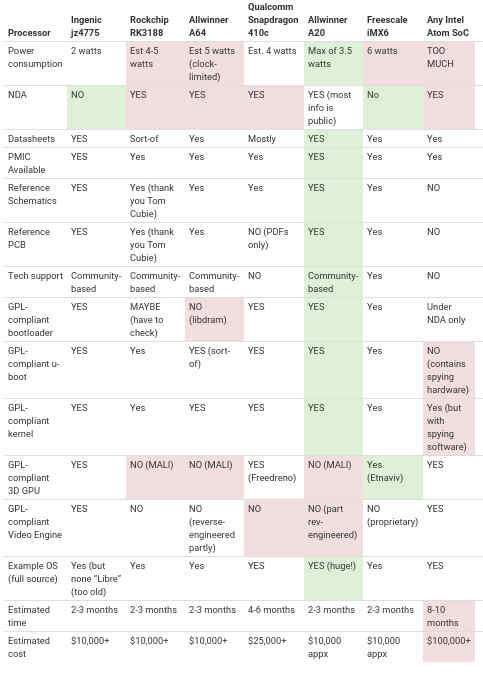
\includegraphics[height=2.4in]{nolibresocs.jpg}\\
  {\bf Analysis of SoCs over the past 7+ years (answer: no)}
 \end{center}
}


\frame{\frametitle{Breakdown of non-existence of fully-Libre SoCs}

 \begin{itemize}
   \item {\bf iMX6}: Libre bootable, Vivante 3D GPU (libre etnaviv)
            but proprietary VPU (and a power-hungry Cortex A9)
	\item {\bf Allwinner SoCs}: mostly Libre bootable,
	      VPU reverse engineered; GPU: MALI or PowerVR (i.e. proprietary)
	\item {\bf Rockchip SoCs}: good but using MALI or PowerVR.
	\item {\bf TI OMAP}: good but using PowerVR.  and expensive.
	\item {\bf Samsung}: good but using MALI.
	\item {\bf Ingenic jz4775}: GREAT! performance
		  sucks (1ghz MIPS32).
	\item {\bf Broadcom SoCs}: Cartelled. and boots from the GPU
  \end{itemize}
  {\it Basically there does not exist one single commercial SoC that
   provides full source code for all functions (CPU, GPU, VPU)
   with modern performance. Which is kinda bizarre if you think about it}
}


\frame{\frametitle{What would a good (Libre) boring, mundane SoC have?}

 \begin{itemize}
   \item Cover a lot of different scenarios (embedded, tablets, industrial,
         netbooks, crypto-currency mining).
	\item Decent performance with high efficiency.  RISC-V: 40\%
		  more efficient than ARM / Intel.  Shakti a good
	      candidate: 2.5ghz and 120mW per core @ 22nm.
	\item 1080p video: y'all gotta watch cute kittens on youtube, right?
	\item 3D GPU: y'all gotta play Angri Burds, right? (or Minecraft)
	\item No spying back-door co-processors (to steal crypto-wallets)
	\item No Spectres, no Meltdowns.
  \end{itemize}
  {\it Basically quite boring and mundane.  No Monster Performance,
   no AI stuff, no special sauce. Just a plain-old SoC,
   40\% more power efficient than ARM/Intel,
   and not spying on end-users, that's all}
}


\frame{\frametitle{How on earth does an ethical Libre SoC make money???}

 \begin{itemize}
   \item Simple answer: Mask Rights.
   \item Without Mask Rights: by having a desirable
         product, and packaging it for a customer (i.e. by being a middle-man
         a service is still being provided for which payment etc. etc.)
   \item Without a desirable product or customer(s): err... you don't.\\
	     (cf: definition of Business)
   \item By not having high NREs (leveraging back-to-back deals,
	     and helping others fulfil their needs and goals)
  \end{itemize}
  {\it Detachment from the goal also helps. If someone else makes this
   product then GREAT! I can go do something else}\\
   \vspace{4pt}
  {\bf Main point: please do not automatically assume Ethical and Libre is
   non-commercial. It's not nice, and it's not helping }

}

\frame{\frametitle{Things wot are "off-limits"}

 \begin{itemize}
   \item Customer entrapment (through proprietary software).\\
         Strong business case for not entrapping customers:\\
	     https://tinyurl.com/most-productive-meeting-ever
   \item Funding, endorsing, supporting or empowering unethical
         Companies, Organisations, Cartels and Individuals.\\
	     (cf: definition of an ethical act).
	\item Being totally inflexible / unrealistic.  Goals have
	     to be met: it's no good being an idiot about that. e.g. if
	     a Libre 3D GPU really can't be made, use Vivante GC800
	     (with etnaviv).
  \end{itemize}
  {\it Still no real show-stoppers to making money (or product):
    it's just slightly harder, that's all.  Ultimately it's about
    confidence. }
}


\frame{\frametitle{Interfaces, Block Diagram, of the Libre-RISCV SoC}
 \begin{center}
  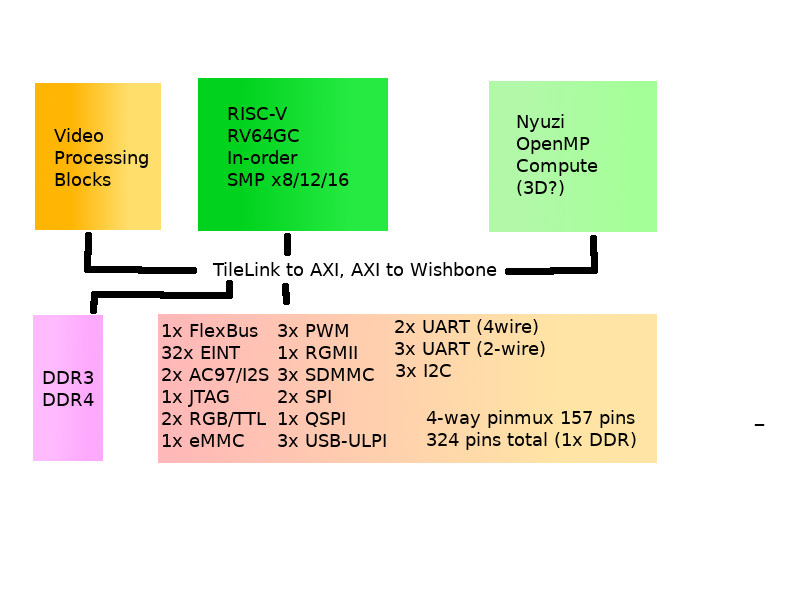
\includegraphics[height=2.1in]{../shakti_libre_riscv.jpg}\\
  {\bf Separate Power Domains for GPIO banks, Variable voltages
    required, low-power sleep states etc.  Quite involved}
 \end{center}
}


\frame{\frametitle{Hardware / Development Complexity Comparison}

 \begin{itemize}
   \item {\bf Server}: relatively easy. PCIe, RapidIO, XAUI, SATA, GbE, 10GE,
		 DDR3/4 (or HMC) etc. etc. No multiplexing: all interfaces dedicated
		 and high-speed differential pairs.
   \item {\bf Desktop}: really just a variant of Server.
	     Graphics is a PCIe Card (except if integrated).  Peripherals
	     often done in dedicated external ICs ("Southbridge" concept)
   \item {\bf Embedded}: also pretty easy.  Really needs a pinmux.  Low clock
         rate, low power mode.  e.g. SiFive Freedom U310.
   \item {\bf Mobile}: HARD. Performance/Watt matters $=>$ variable core
		 voltage domains {\it per core}.  Number of pins matters (affects
		 yield and package cost).  Cost
		 matters.  Pinmux critical.
  \end{itemize}
  {\it Bottom line: Mobile-class processors are challenging!}
}


\frame{\frametitle{Proprietary vs Libre-licensed Interface HDL}

 \begin{itemize}
   \item DDR3/4: challenging! \$1m for single-use, single instance.\\
         Symbiotic EDA: \$600k for PHY; CERN developed a Controller\\
         http://libre-riscv.org/shakti/m\_class/DDR/
   \item HyperRAM (JEDEC xSPI): lower risk than DDR3/4\\
	   http://libre-riscv.org/shakti/m\_class/HyperRAM/
   \item RGMII: several available (saves \$50k)\\
	   http://libre-riscv.org/shakti/m\_class/RGMII/
   \item UART, SPI, I2C, PWM, SD/MMC: all libre (except eMMC).
   \item Shakti Group has FlexBus, QuadSPI, SRAM, many more.
   \item RGB/TTL: R. Herveille (SSD2828, SN75LVDS83b, TFP410a)
  \end{itemize}
  {\it Basically there's no compelling reason to spend vast sums
   on proprietary HDL.  Sorry Cadence / Mentor / Synopsis / whoever}
}


\frame{\frametitle{Challenging Stuff [1] - Memory Interfaces}

 \begin{itemize}
   \item DDR3/4 PHYs are analog and very high speed.
		   Impedance training.  Extreme timing tolerances on parallel buses.\\
		   No surprise proprietary cost is USD \$1m and above.
   \item Symbiotic EDA will do (Libre) PHY layout for USD \$300k,
	     time to completion for chosen geometry: 8-12 months.
  \end{itemize}
   {\it Silicon-proven but still risky.  What are the alternatives?}
   \vspace{4pt}
 \begin{itemize}
   \item 133mhz 32-bit SDRAM (um...) maybe even FlexBus?
   \item HyperRAM (aka JEDEC xSPI) 8-bit SPI 166mhz or DDR-300.\\
	   300mbyte/sec for only 13 wires, not bad!  (We'll take several)\\
	   http://libre-riscv.org/shakti/m\_class/HyperRAM/
   \item HMC: insanely fast, very low power.  OpenHMC (LGPL)
	   https://opencores.org/project/openhmc
  \end{itemize}
}


\frame{\frametitle{Challenging Stuff [2] - Video Decode Engine}

 \begin{itemize}
   \item Richard Herveille's Video Core Blocks\\
    	    https://opencores.org/project/video\_systems
   \item Symbiotic EDA MP4 decoder in FPGA
   \item H.264 seems to have been done...\\
         https://github.com/adsc-hls/synthesizable\_h264
   \item Really needs SIMD (or better, not-SIMD)\\
         {http://libre-riscv.org/simple\_v\_extension/}
   \item Definitely needs xBitManip (parallelised by Simple-V)\\
         https://github.com/cliffordwolf/xbitmanip
  \end{itemize}
   {\it SIMD is insane. $O(N^6)$ opcode proliferation.  See\\
     https://www.sigarch.org/simd-instructions-considered-harmful/ \\
     (1): P-Ext designed for Audio. (2): Investigate RI5CY's SIMD
   }
}


\frame{\frametitle{Challenging Stuff [3] - Power Management}

 \begin{itemize}
   \item Been done before (many times), but not as a Libre Design.
   \item Sanjay Charagulla: GlobalFoundries 22nm mobile process
	     can reach as low as 0.4v
   \item GPIO Banks need per-bank VREF (1.8v? to 3.3v)\\
	      IO pads need built-in
	     level-shifting to convert to CPU VCORE
   \item Each core needs independent variable-voltage capability
	     and independent shut-down (PMIC supplies external voltage)
   \item DDR RAM still needs refreshing (even in sleep mode)
   \item Extra RV32 (PicoRV32?) always-on core for wake-up / RTC?
   \item PLLs are Analog.  fun fun fun in the sun sun sun...
  \end{itemize}
   {\it Really need help.  PLLs, Analog stuff: specific
	   domain expertise.  Fall-back example:
	   https://www.dolphin-integration.com?
   }
}


\frame{\frametitle{Challenging Stuff [4] - Libre 3D GPU.  Sigh.}

 \begin{itemize}
   \item Actual requirements quite modest: 30MP/s 100MT/s 5GFLOPS
         but power/area is crucial ($2mm^2$ @ 40nm)
   \item Nyuzi, MIAOW, GPLGPU (Number Nine), OGP.
   \item Nyuzi based on Larrabee. Jeff Bush really helpful.
   \item MIAOW is an OpenCL engine.  GPLGPU is fixed-function
   \item Nyuzi lessons: Software-only rendering not enough.
	     Getting through L1 cache takes most power. Fixed functions
	     such as parallel FP-Quad to ARGB Pixel, and Z-Buffer
	     needed.
   \item Fallback is GC800 (\$250k) {\it contact me if you can do better!}
  \end{itemize}
   {\it Jacob Bachmeyer's Cache-control proposal turns L1 Cache into
   scratchpad RAM.  RVV is just too heavy (sorry!), Simple-V much
   more light-weight and flexible ($O(1)$ ISA proliferation)
   }
}


\frame{\frametitle{Challenging Stuff [5] - Custom Extensions}

 \begin{itemize}
   \item GPUs are usually done with incompatible ISAs and effectively
	     doing OpenGL over IPC / RPC (Remote Procedure Calls)
   \item Much simpler: GPGPU approach.  Custom-extend the 
	     main core ISA to handle 3D, and accelerate
		 Gallium3D-LLVM. 
   \item Now add Video Extensions. and SIMD. and, and, and...\\
	   {\bf we are well beyond the 2 32-bit custom opcodes}
   \item Due to the Libre nature of this project, the custom opcode
	     space will be "dominated" by 
	     high-profile public hard-forks of gcc, binutils, llvm etc.
	     Which isn't going to go down well.
   \item ISA "Conflict Resolution" is therefore absolutely critical\\
	     http://libre-riscv.org/isa\_conflict\_resolution/
  \end{itemize}
   {\it Remember Altivec. Learn from Intel.
   \underline{This is everyone's problem.}
   }
}


\frame{\frametitle{TODO}

 \begin{itemize}
   \item TODO\vspace{8pt}
  \end{itemize}
}


\frame{\frametitle{Summary}

 \begin{itemize}
   \item Making a commercially-desirable SoC is neither academically
         nor standard-investor sexy!  No AI. Boring. zzzz
   \item Luckily there is an anonymous sponsor who needs an SoC that
	     doesn't exist (who knows the commercial benefits of Libre)
   \item Shakti Group know the benefits (cost, sovereignty) of a Libre
         Mobile-Class SoC as well (No spying on India citizens!)
   \item A Libre GPU, even a modest performer (100T/s etc.) 
	     is the biggest technical risk/unknown (besides DDR3/4).\\
	     (fall-back is GC800. Do please help with a Libre GPU!)
    \item DDR3/4 and eMMC are the main high-risk interfaces\\
	     (there are fall-back strategies in place)
	\item Ultimately the strategy is all about cost reduction
	      vs risk mitigation,
	      with Libre/Ethical prioritised over "convenience"
  \end{itemize}
}


\frame{
  \begin{center}
    {\Huge The end\vspace{20pt}\\
		   Thank you\vspace{20pt}\\
		   Questions?\vspace{20pt}
	}
  \end{center}
  
  \begin{itemize}
	\item Contact: lkcl@lkcl.net 
	\item http://libre-riscv.org/shakti/m\_class/
  \end{itemize}
}


\end{document}
